\begin{center}
    \textbf{Вариант №1}
\end{center}

\paragraph{Блок-схемы классов}

Блок-схема наследования классов изображена на рисунке \ref{fig:task-variant-1} (стр. \pageref{fig:task-variant-1}).

\begin{figure}[!htp]
    \center{
        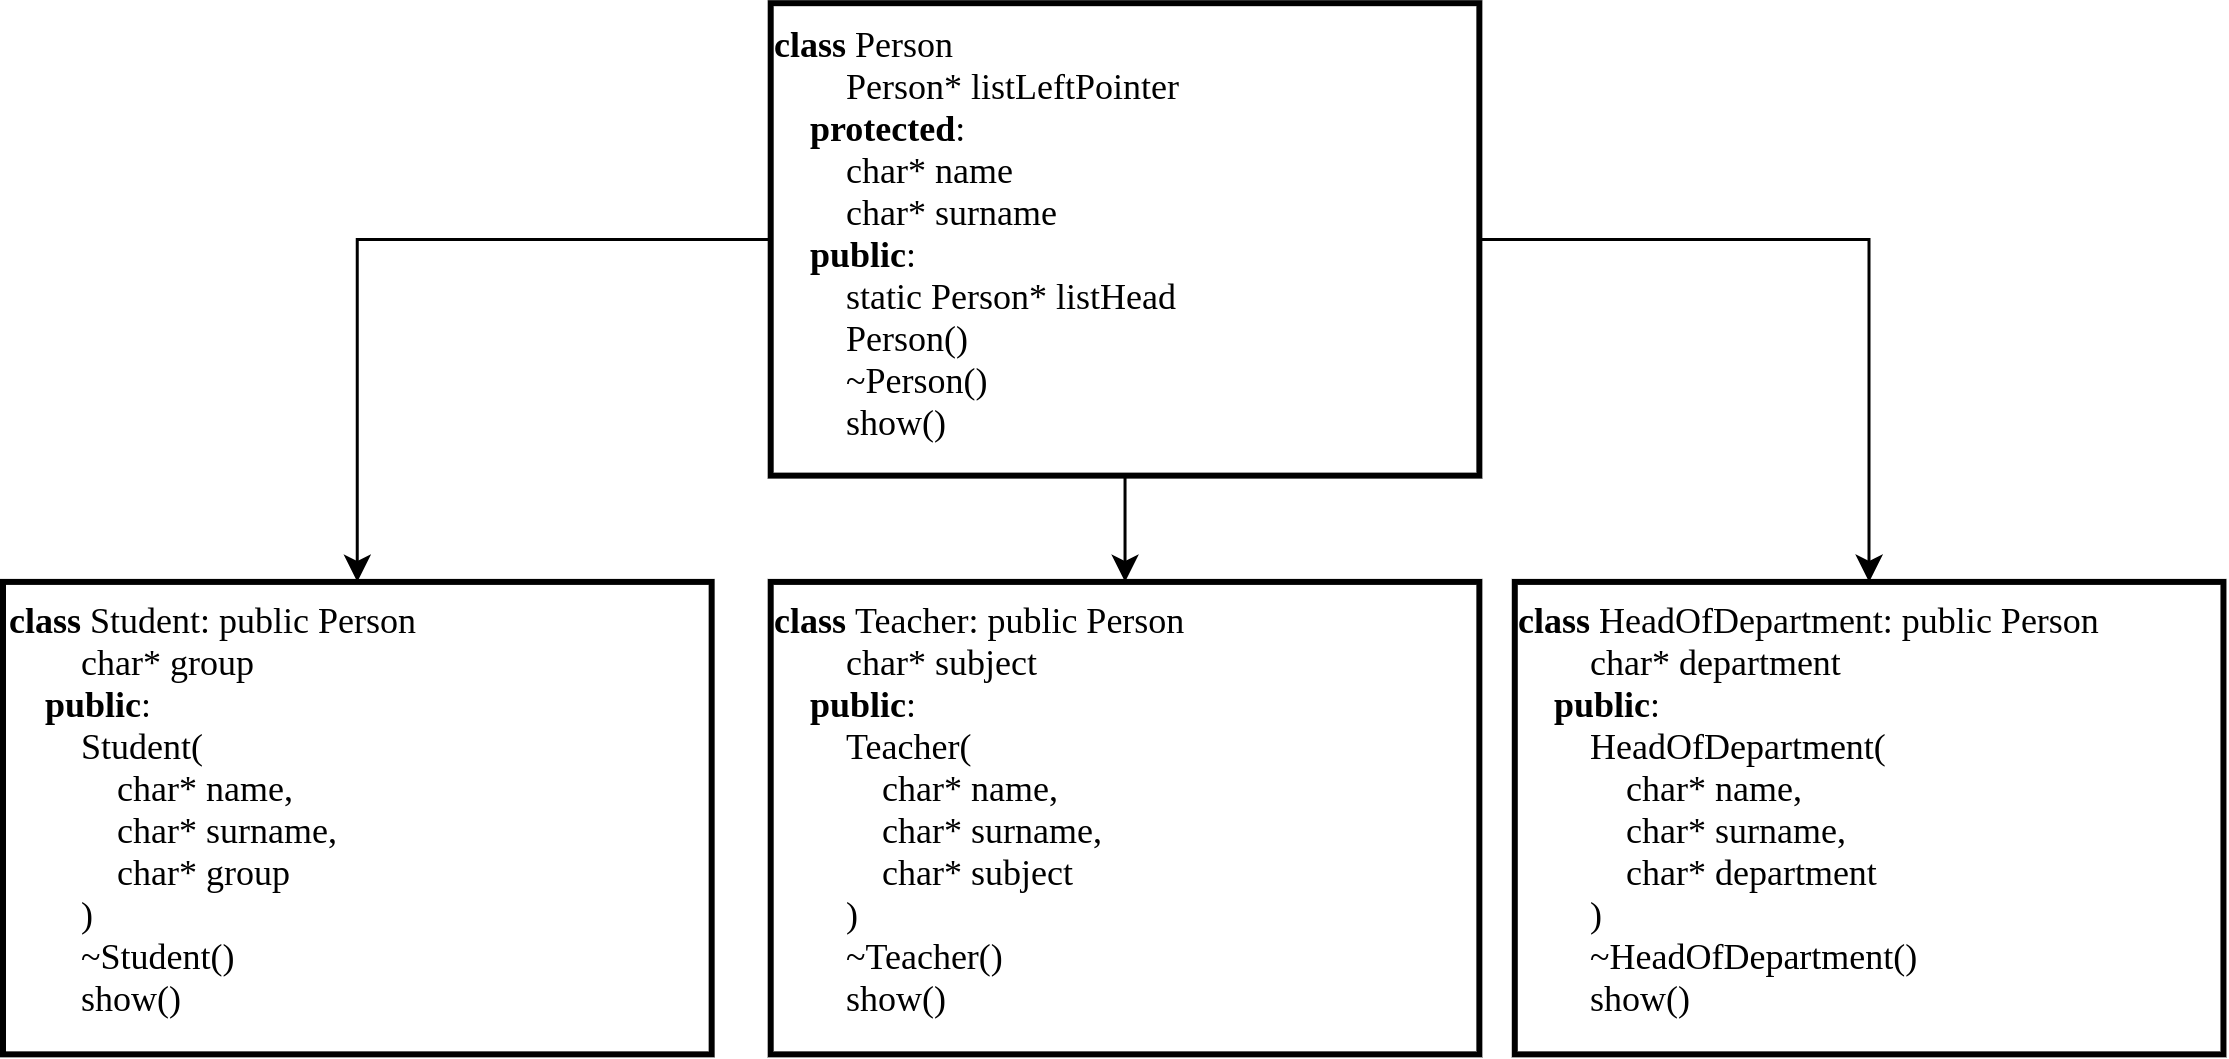
\includegraphics[width=10cm]
        {../../src/option1/src/Person/Person.png}
    }
    \caption{Наследование классов}
    \label{fig:task-variant-1}
\end{figure}

\lstinputlisting[language=C++, name=main.hpp,]
{../../src/option1/src/main.hpp}

\lstinputlisting[language=C++, name=main.cpp,]
{../../src/option1/src/main.cpp}

\newpage

\lstinputlisting[language=C++, name=Person.hpp,]
{../../src/option1/src/Person/Person.hpp}

\lstinputlisting[language=C++, name=Person.cpp,]
{../../src/option1/src/Person/Person.cpp}

\newpage

\lstinputlisting[language=C++, name=Student.hpp,]
{../../src/option1/src/Person/Student/Student.hpp}

\lstinputlisting[language=C++, name=Student.cpp,]
{../../src/option1/src/Person/Student/Student.cpp}

\newpage

\lstinputlisting[language=C++, name=Teacher.hpp,]
{../../src/option1/src/Person/Teacher/Teacher.hpp}

\lstinputlisting[language=C++, name=Teacher.cpp,]
{../../src/option1/src/Person/Teacher/Teacher.cpp}

\newpage

\lstinputlisting[language=C++, name=HeadOfDepartment.hpp,]
{../../src/option1/src/Person/HeadOfDepartment/HeadOfDepartment.hpp}

\lstinputlisting[language=C++, name=HeadOfDepartment.cpp,]
{../../src/option1/src/Person/HeadOfDepartment/HeadOfDepartment.cpp}

\newpage

\begin{lstlisting}[language=Out,]
[
    {
        "name": "Vladimir",
        "surname": "Golovko",
        "department": "Intelligent information technology",
    },
    {
        "name": "Alexander",
        "surname": "Kroshchenko",
        "subject": "Decision making methods and algorithms",
    },
    {
        "name": "Oksana",
        "surname": "Voitsekhovich",
        "subject": "Interface and software development technologies",
    },
    {
        "name": "Ivan",
        "surname": "Gladki",
        "subject": "Hight Math",
    },
    {
        "name": "Tatiana",
        "surname": "Glushchenko",
        "subject": "Discrete Math",
    },
    {
        "name": "Maria",
        "surname": "Khatskevich",
        "subject": "Programming languages",
    },
    {
        "name": "Sergey",
        "surname": "Anfilets",
        "subject": "Programming languages",
    },
    {
        "name": "Ilya",
        "surname": "Yakovchik",
        "group": "PS-4",
    },
    {
        "name": "Vladislav",
        "surname": "Yuriev",
        "group": "PS-4",
    },
    {
        "name": "Anastasia",
        "surname": "Shiba",
        "group": "PS-4",
    },
    {
        "name": "Denis",
        "surname": "Typik",
        "group": "PS-4",
    },
    {
        "name": "Danil",
        "surname": "Sinyak",
        "group": "PS-4",
    },
    {
        "name": "Nikita",
        "surname": "Prokopyuk",
        "group": "PS-4",
    },
    {
        "name": "Nikolay",
        "surname": "Pivnik",
        "group": "PS-4",
    },
    {
        "name": "Alexander",
        "surname": "Mayevsky",
        "group": "PS-4",
    },
    {
        "name": "Alexey",
        "surname": "Lud",
        "group": "PS-4",
    },
    {
        "name": "Alexey",
        "surname": "Kydzela",
        "group": "PS-4",
    },
    {
        "name": "Kirill",
        "surname": "Krechko",
        "group": "PS-4",
    },
    {
        "name": "Stanislav",
        "surname": "Kotashevich",
        "group": "PS-4",
    },
    {
        "name": "Vladislav",
        "surname": "Kovalchuk",
        "group": "PS-4",
    },
    {
        "name": "Vladimir",
        "surname": "Kalinovsky",
        "group": "PS-4",
    },
    {
        "name": "Ivan",
        "surname": "Ivanenko",
        "group": "PS-4",
    },
    {
        "name": "Zhuk",
        "surname": "Vladislav",
        "group": "PS-4",
    },
    {
        "name": "Sergey",
        "surname": "Eliseev",
        "group": "PS-4",
    },
    {
        "name": "Alexandra",
        "surname": "Gritsak",
        "group": "PS-4",
    },
    {
        "name": "Dmitry",
        "surname": "Gribovsky",
        "group": "PS-4",
    },
    {
        "name": "Pavel",
        "surname": "Galanin",
        "group": "PS-4",
    },
    {
        "name": "Anastasia",
        "surname": "Vorobey",
        "group": "PS-4",
    },
    {
        "name": "Maxim",
        "surname": "Borovsky",
        "group": "PS-4",
    },
    {
        "name": "Yana",
        "surname": "Baiduk",
        "group": "PS-4",
    },
    {
        "name": "Daniil",
        "surname": "Andreychikov",
        "group": "PS-4",
    },
    {
        "name": "_",
        "surname": "_",
    },
]       
\end{lstlisting}

\paragraph{Вывод:}
Научились делать наследование.
Реализовали три класса (Student, Teacher, HeadOf Department), которые наследую один класс (Person).
Для троих классов (Student, Teacher, HeadOfDepartment) переопределили метод show, но чтобы он переопределялся, то использовали virtual в базовом классе (Если в базовом классе вызывается show, а это другой класс, который просто наследует этот, то чтобы не вызывался базовый метод прописали виртуал).
Для базового класса (Person) реализовали динамическую структура данных <<Список>>, используя статический указатель на голову (чтобы во всех классах была известна одна голова списка), статический размер списка (чтобы во всех класса была информация о размере списка).